\newpage
\chapter{TINJAUAN PUSTAKA} \label{Bab II}

\section{Tinjauan Pustaka} \label{II.Tinjauan}
Penulis  melakukan  pencarian  referensi  terkait beberapa penelitian serupa yang pernah dilakukan sebagai dasar penelitian. Penelitian-penelitian yang menjadi referensi penulis dijabarkan pada Tabel \ref{table:2.literasi}. \par
\renewcommand{\arraystretch}{1.0} % Mengatur spasi antar baris menjadi 1
\begin{longtable}{|c|p{0.25\textwidth}|p{0.21\textwidth}|p{0.145\textwidth}|p{0.2\textwidth}|}
  \caption{Literasi Penelitian Terdahulu}\label{table:2.literasi}\\
  \hline
  \textbf{No} 
    & \textbf{Penulis [Tahun] [Judul]} 
    & \textbf{Permasalahan} 
    & \textbf{Metode} 
    & \textbf{Hasil} \\ % ← you must end the row here
  \hline
\endfirsthead
  \hline
  \textbf{No} 
    & \textbf{Penulis [Tahun] [Judul]} 
    & \textbf{Permasalahan} 
    & \textbf{Metode} 
    & \textbf{Hasil} \\ % ← and here too
  \hline
\endhead
  \hline
\endfoot
  \hline
\endlastfoot
    1. & Weibo Wang, Zongkai Wei, Jin Yuan, Yu Fang, dan Yongkang Zheng [2022] [Non-contact heart rate estimation based on singular spectrum component reconstruction using low-rank matrix and autocorrelation] & akaoapaoaj & ak & \\ 
    \hline
    2. & Riza Agung Firmansyah, Yuliyanto Agung Prabowo, Titiek Suheta, dan Syahri &  &  & \\
    \hline
    & [2023] [Implementation of 1D convolutional neural network for improvement remote photoplethys-mography] & & & \\ 
\end{longtable}




\section{Dasar Teori} \label{II.Teori}
Berikut ini merupakan dasar teori yang digunakan pada penelitian ini: \par

\subsection{Teori 1} \label{II.teori1}
Denyut yang dirasakan sebenarnya bukan darah yang dipompa langsung oleh jantung ke aorta, melainkan gelombang tekanan yang berasal dari aorta yang merambat lebih cepat dibandingkan aliran darah itu sendiri \cite{Ivanny2014Perbandingan}. \par


\subsection{\textit{Teori 1}} \label{II.teori2}
\lipsum[1-2] % Menampilkan paragraf 1 sampai 2 dari lorem ipsum
Gambar yang digunakan \ref{fig:3.ref_gbr}. \par
\begin{figure}[H] % Kalau menggunakan H, posisi gambar akan tepat dibawah teks
    \centering
    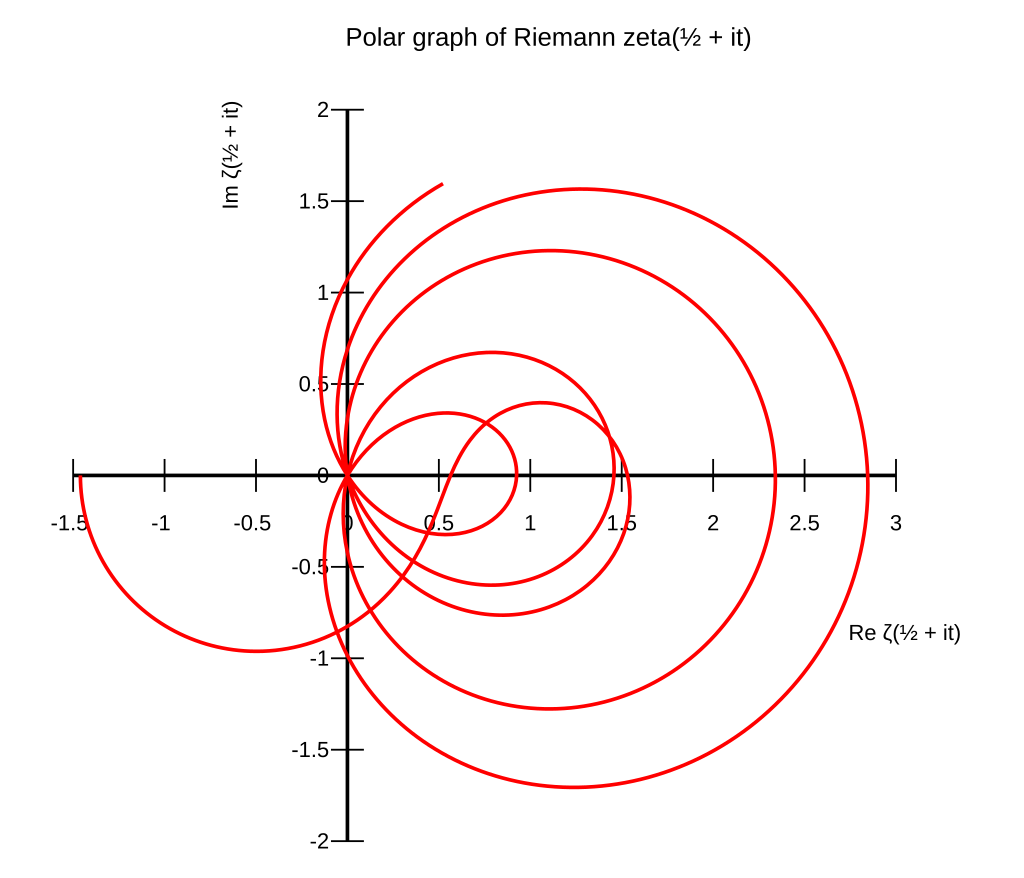
\includegraphics[width=0.6\textwidth]{figure/zeta.png}
    \caption{Referensi Gambar}
    \label{fig:3.ref_gbr}
    {\footnotesize Sumber: internet}
\end{figure}

\subsection{\textit{Teori 2}} \label{II.teori3}
\lipsum[3-4] % Menampilkan paragraf 3 sampai 4 dari lorem ipsum
Berikut adalah ilustrasi konsep yang digunakan seperti pada Gambar \ref{fig:3.ref_gbr2}. \par
\begin{figure}[H] % Posisi gambar tepat dibawah teks
  \centering
  
\includegraphics[width=0.7\textwidth]{figure/Logo_ITERA.png}
  \caption{Ilustrasi Konsep}
  \label{fig:3.ref_gbr2}
  {\footnotesize Sumber: dokumentasi penelitian}
\end{figure}

\subsection{Metrik Performa: MAE, RMSE} \label{II.mae}
\textit{Mean Absolute Error} (MAE) \cite{Suryanto2019MAE} \cite{cort2005maermse}. Rumus perhitungan dari MAE dapat dilihat pada \ref{eq:2.mae}. \par

\begin{equationcaptioned}[eq:2.mae]{
    MAE = \frac{1}{n} \sum_{i=1}^{n} \left| y_i - \hat{y}_i \right|
}{
    Mean Absolute Error (MAE)
}
\end{equationcaptioned}